\documentclass[conference]{IEEEtran}
\usepackage{cite}
\usepackage{amsmath,amssymb}
\usepackage{graphicx}
\usepackage{booktabs}
\usepackage{textcomp}
\usepackage{xcolor}
\usepackage{url}

\newcommand{\mi}{\textminus}
\newcommand{\BD}{B+D}
\newcommand{\BDT}{B+D+T}

\begin{document}

\title{Does Topology Help Ring Detection? Directed Flag Persistence Against Direction and Behaviour Features on Transaction Graphs}

\author{\IEEEauthorblockN{Niharika K P, Priyadarshini Prasad,\\
Nidhi Santosh Nayak, Nischita M}
\IEEEauthorblockA{\textit{School of Computer Science and Engineering}\\
\textit{RV University}\\
Bengaluru, India\\
niharikakpbtech25@rvu.edu.in, priyadarshiniprasadbtech25@rvu.edu.in,\\
nidhisantoshnayakbtech25@rvu.edu.in, nischitambtech25@rvu.edu.in}}

\maketitle

\begin{abstract}
Wash trading and laundering cycles appear as directed loops among a few accounts, not as unusual single transactions. We ask whether topological features of those loops add predictive value over graph-baseline features (B) and direction and behaviour features (D, which include the ring's birth value in a suspicion-weighted filtration). Each time window becomes a weighted directed graph. Candidate rings are enumerated exactly inside strongly connected components, and persistent homology of a directed flag complex of each ring's neighbourhood gives topological features (T). The comparison B+D+T versus B+D was fixed before the experiments and is judged by paired grouped-bootstrap intervals. On the IBM AML benchmark (itself synthetic) we find no detectable topological lift within either dataset: for logistic regression on HI-Small the paired PR-AUC difference is +0.104 [\mi0.002, +0.171] with 14 positive groups, and LI-Small (10 positive groups) agrees in that every interval includes 0; the intervals cannot rule out a small effect either way. In transfer between the two datasets, B+D+T is below B+D in two of six primary cells, with intervals that exclude 0. Direction and behaviour features carry the detection signal. On a synthetic generator that is nearly separable by D, a small lift appears in 7 of 12 condition-model cells, not where the design predicted, and it does not carry to IBM. The ring-birth score that works on HI-Small (0.314) does not replicate on LI-Small (0.006); these are two separate no-model scores, one per dataset. In simulation, discounted-UCB and sliding-window Thompson bandit thresholds lose to periodic re-tuning, while online gradient ascent reaches 0.981 of the hindsight oracle in simulation. A real-data NFT experiment was not run.
\end{abstract}

\begin{IEEEkeywords}
wash trading, anti-money laundering, persistent homology, directed flag complex, graph anomaly detection, negative results
\end{IEEEkeywords}

%--------------------------------------------------------------------
\section{Introduction}
\label{sec:intro}

Wash trading means trading with oneself through a front: colluding accounts pass an asset or money around so that the last recipient hands it back to the first. Nothing economic happens, but recorded volume rises. Measurement studies find it on decentralized exchanges and in NFT markets \cite{victor2021wash,tosic2025beyond,liu2023nft}, and a recent working paper reports it on a prediction-market exchange \cite{sirolly2025network}. Laundering through layering has the same shape, with value cycling through intermediaries. In both cases every payment looks ordinary. What is unusual is a loop: a small group of accounts in which value circulates and nets to about zero for each member.

Two gaps motivate this work. First, detectors built around dense subgraphs, communities or node centrality look for tightly connected groups, while a ring can be sparse, with each member trading with only two or three others. Cycle enumeration finds such loops but returns a binary answer with no measure of strength, stability or type. Second, flagging thresholds tuned once on history lose accuracy when manipulators change ring size, timing and decoy trades.

Persistent homology gives a continuous description of loops. In a \emph{directed} flag complex a circular triangle $a\to b\to c\to a$ is never filled, so its loop persists, while a transitive triangle $a\to b$, $b\to c$, $a\to c$ is filled at once \cite{lutgehetmann2020flagser}. We apply this complex to candidate rings and ask a deliberately narrow question: \emph{given the ring's direction and behaviour features, do topological features add predictive value?} Ring birth, the largest edge weight on the ring, is a function of the ring's own edges, so we count it in the direction and behaviour set D and not in the topological set T. The primary comparison, fixed in advance, is B+D+T against B+D, where B are graph-baseline features. Because only 10 to 14 positive groups exist in the IBM data (itself synthetic), we report intervals as they are and tune nothing to narrow them.

\textbf{Scope.} The target is the closed cycle: wash-trading rings and laundering cycles of up to six accounts. Pump-and-dump coordination is a temporal motif and not a cycle; it appears only as a small synthetic track without topology. Spoofing is out of scope, because it is an order-book phenomenon with no signal in settled transactions. We evaluate on the IBM AMLworld benchmark, which is synthetic, and on our own synthetic generator with planted rings; no real market data were used.

\textbf{Contributions.}
\begin{enumerate}
\item A suspicion-weighted filtration and a directed-flag-complex pipeline for candidate rings, with exact account-level localization by cycle enumeration, two persistence backends that agree within tolerance, and an exact test of whether a ring's own loop is ever filled. We claim no priority for applying directed flag complexes to transaction graphs.
\item A pre-specified comparison of B+D+T and B+D under group-aware cross-validation. On IBM AML data (itself synthetic) there is no detectable topological lift within either dataset and the intervals cannot exclude a small effect either way; in transfer between the datasets two of six primary cells are negative with intervals excluding 0. D clearly beats B.
\item On a synthetic generator nearly separable by D, a small lift in 7 of 12 condition-model cells that is not concentrated where the design predicted and that does not carry to IBM; and a ring-birth signal that does not replicate on LI-Small (0.314 on HI-Small, 0.006 on LI-Small; two separate no-model scores).
\item Documented exploratory and negative results: bandit thresholds that lose to periodic re-tuning, a severity regression that recovers generator structure, weak clustering by pattern type, and small sensitivity to the infinite-bar cap among the pre-set rules (at most 0.024 in PR-AUC).
\end{enumerate}

Section~\ref{sec:related} places the work among existing detectors, Section~\ref{sec:method} describes the pipeline, Section~\ref{sec:setup} the data and protocol, Section~\ref{sec:results} the results, and Section~\ref{sec:discussion} the limitations, including what was not done.

%--------------------------------------------------------------------
\section{Related Work}
\label{sec:related}

\textbf{Wash-trade measurement and rules.} Empirical studies identify wash trading by rules over accounts and trades. On two order-book decentralized exchanges, Victor and Weintraud find a lower bound of 159 million USD wash-traded, more than 30\% of tokens affected, and structures that mostly involve one or two accounts \cite{victor2021wash}. On seven NFT collections a repurchase rule (a wallet buys back a token within 30 days of selling it) flags on average 0.14\% of transactions \cite{liu2023nft}, while linking NFT ownership traces to the full Ethereum transaction network finds wash trading up to 24\% of volume, with one outlier collection at 93\% \cite{tosic2025beyond}. For stock markets, Cao et al.\ model collusion as a directed trader graph over matched orders and solve two knapsack-like steps by dynamic programming \cite{cao2016wash}. Sirolly et al.\ assume wash traders form nearly closed clusters of counterparties and apply an iterative network procedure to a prediction market; their paper is a working paper and not peer reviewed \cite{sirolly2025network}. These methods see self-trades, short cycles and closed clusters. None assigns a ring a continuous strength from a filtration, and none is evaluated here, so we make no comparative claim.

\textbf{Graph and learning detectors for fraud and AML.} Dense-subgraph detection under camouflage is addressed by Fraudar on bipartite review graphs \cite{hooi2017fraudar}. For laundering, Weber et al.\ release a labelled Bitcoin graph and report that random forest outperforms graph convolutional networks \cite{weber2019aml}; Ouyang et al.\ classify laundering groups with subgraph contrastive learning \cite{ouyang2024bitchetg}; Pei et al.\ embed subgraphs by structural roles and score them with Isolation Forest, restricting themselves to undirected, unweighted networks \cite{pei2020sade}. Chen et al.\ shrink strongly connected components and run a parallel depth-first search to mark suspicious accounts \cite{chen2023parallel}. Learned detectors need labels and tuning and give little per-loop interpretation; component-and-search methods localize loops but return a binary answer. We use classical classifiers only and did not compare against graph neural networks.

\textbf{Cycle enumeration.} We localize rings by enumerating simple directed cycles up to a length bound with NetworkX \cite{networkx_simple_cycles}, whose documentation names Johnson's algorithm for the unbounded case \cite{johnson1975circuits} and a version of the algorithm of Gupta and Suzumura for the bounded case \cite{gupta2021bounded}. A recent preprint presents examples in which the latter fails to enumerate valid cycles \cite{bauernoppel2025bounded}; we did not test our enumeration against it, so our candidate recall may be affected in a way unrelated to the parameters we vary.

\textbf{Topology on graphs.} Ofori-Boateng et al.\ track the shape of multilayer blockchain graphs with clique persistent homology and report gains over state-of-the-art baselines for network-level anomalies \cite{ofori2021topological}. A clique complex ignores direction, and it describes the network as a whole, not individual rings. Directed flag complexes and their persistent homology are computed by flagser, developed for brain-network data \cite{lutgehetmann2020flagser}; tournaplexes refine them by filling non-transitive cliques and distinguish graph dynamics more finely on the same kind of data \cite{govc2021tournaplex}. Persistence diagrams must be vectorized for classifiers; we use persistence landscapes \cite{bubenik2015landscapes} with fixed settings, and note that learned weighting of persistence summaries exists \cite{zhao2019wkpi} but was not tried. Our contribution here is a controlled test of what such features add for per-ring classification, not a new topological construction.

\textbf{Drift and thresholds.} Streaming fraud detection often uses drift detectors to decide when to retrain \cite{vivek2025rosfd}. Bandits for changing reward distributions include discounted UCB \cite{garivier2011switching} and sliding-window Thompson sampling \cite{trovo2020swts}, whose analysis has since been revisited and corrected in a preprint \cite{fiandri2024swts}. We simulate only, on one synthetic drift stream.

\textbf{Data.} The IBM AMLworld generator provides laundering data with complete labels \cite{altman2023realistic}; SynthAML is a different synthetic AML benchmark built from real bank data \cite{jensen2023synthaml}, which we did not use. Temporal-motif analyses of cryptocurrency graphs show that whole-network counts can mislead and that per-user and per-period views reveal more \cite{arnold2024motifs}, which is one reason we work with time windows and local neighbourhoods.

\textbf{Where this work sits.} Across these families a loop is either found and reported as binary, or described by network-level or node-level statistics. We keep exact enumeration as the localizer, because the persistence library interface we use cannot name the accounts of a loop, and ask a narrower question about the features: whether a per-ring persistence description helps once the ring's own weights and behaviour and the surrounding graph are already known. The design choices that make the answer interpretable are that ring birth is placed in D and not credited to topology, that the baseline sees at least as much of the graph as T does, and that rings are grouped so that near-copies never straddle a split. We did not run the other methods named above, and make no claim about them.

%--------------------------------------------------------------------
\section{Method}
\label{sec:method}

Figure~\ref{fig:pipeline} summarizes the pipeline.

\begin{figure*}[t]
\centering
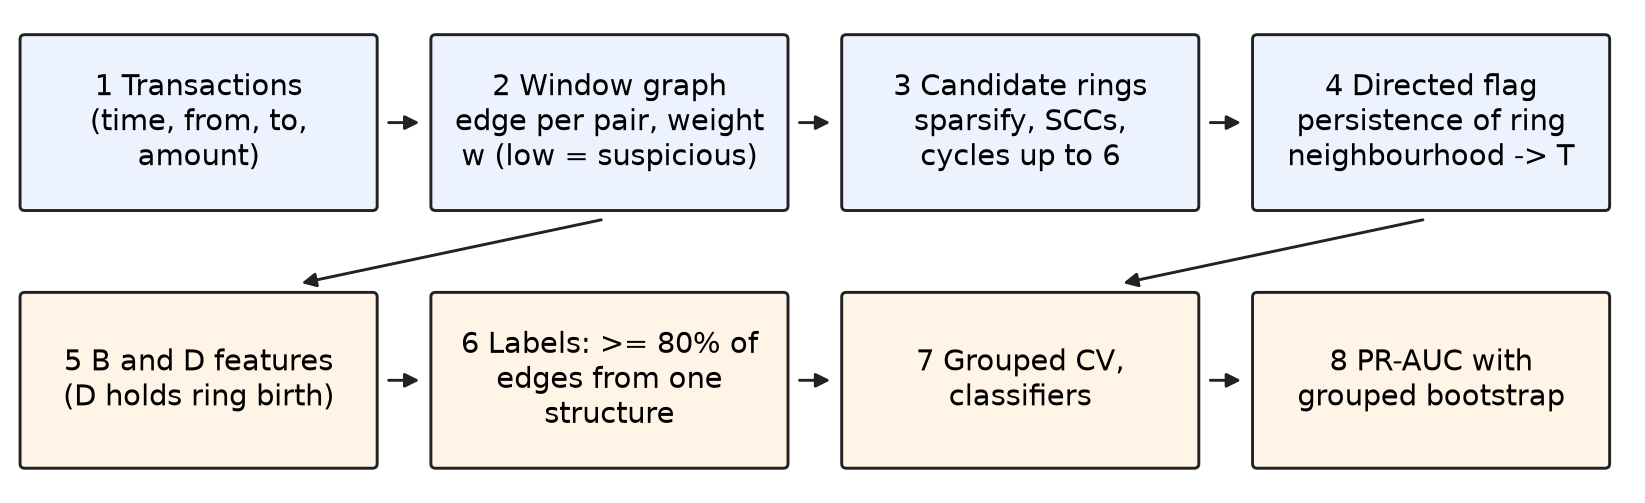
\includegraphics[width=\textwidth]{figures/f1_pipeline.png}
\caption{Pipeline from transactions to out-of-fold PR-AUC. Blue: graph and topology stages; orange: features, labels and evaluation. The compared feature sets are B, B+D, B+D+T and T; the pre-specified primary comparison is B+D+T against B+D.}
\label{fig:pipeline}
\end{figure*}

\subsection{Windows, scores and weights}
Time is cut into windows (5 days with a 1-day stride on IBM data). Within a window all payments from $a$ to $b$ form one directed edge carrying total volume $V_{ab}$, count, and the coefficient of variation (CV) of inter-payment gaps. Three scores lie in $[0,1]$, higher meaning more suspicious. Pair reciprocity is $s_{\mathrm{rec}}=1-|V_{ab}-V_{ba}|/(V_{ab}+V_{ba})$. Node flow balance is $s_{\mathrm{bal}}=\min(\beta(a),\beta(b))$ with $\beta(x)=1-|\mathrm{in}_x-\mathrm{out}_x|/(\mathrm{in}_x+\mathrm{out}_x)$. Timing regularity is $s_{\mathrm{reg}}=1/(1+\mathrm{CV})$; pairs with fewer than three payments have no CV and receive the window median. Each score is replaced by its rank within the window, scaled to $[0,1]$, with ties taking the lowest rank. The edge weight is $w=1-\mathrm{mean}$ of the three ranked scores, so \emph{a lower weight is more suspicious}, matching the sublevel-set filtration in which low-weight cells enter first.

\emph{Proposition 1.} In a ring of three or more accounts with no reciprocal pair, the ranked $s_{\mathrm{rec}}$ is 0 on every edge, so under equal weights $w\ge 1/3$ however balanced and regular the ring is. A multi-party ring cannot look maximally suspicious under equal weights, which motivates learning the combination weights on the probability simplex (Appendix~\ref{app:report}).

\subsection{Candidate rings}
A candidate generator keeps edges with $w\le\tau$ (a quantile of the window's weights: 0.05 on IBM, 0.25 on synthetic data), computes strongly connected components, and enumerates simple directed cycles of length at most 6, with a cap of 20{,}000 cycles per component whose hits are recorded. Each cycle is an explicit set of accounts and edges. Its \emph{birth} is the largest edge weight on it. De-duplication, as implemented, removes nothing for maximum length up to 9, so near-duplicate rings all remain candidates; the evaluation therefore groups them (Section~\ref{sec:setup}). Localization is combinatorial because the pyflagser interface we use returns persistence pairs but no representative cycles.

\subsection{Directed flag persistence}
For a candidate we take the ring plus its one-hop neighbours in the sparsified graph and build the weighted directed flag complex up to dimension 2: vertices at 0, directed edges at their weight, and a 2-cell for each ordered triple $(a,b,c)$ with edges $a\to b$, $a\to c$, $b\to c$ at the largest of the three weights. H0 and H1 diagrams come from flagser (float32) or a pure-Python $\mathbb{Z}/2$ reduction; the two must agree within tolerance, and tests check the canonical cases (Fig.~\ref{fig:triangles}). The diagram of the whole sparsified window is computed once per window.

\begin{figure}[t]
\centering
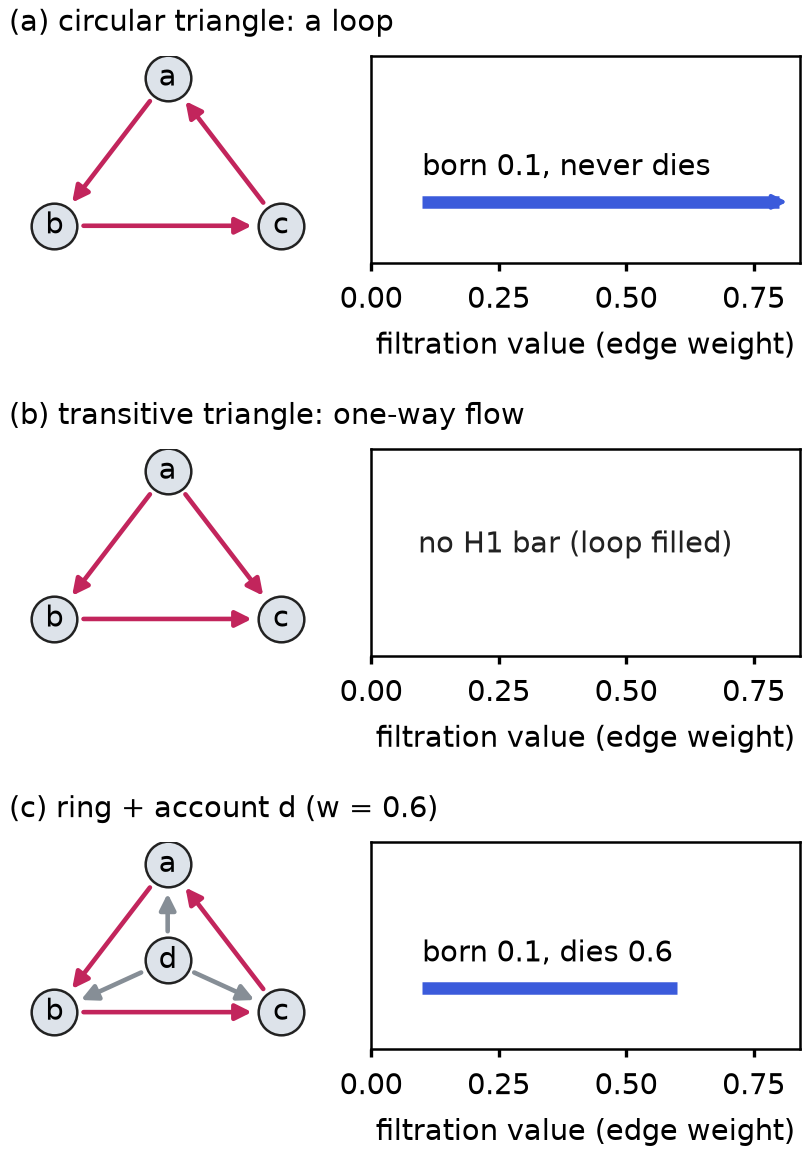
\includegraphics[width=0.78\columnwidth]{figures/f2_triangles.png}
\caption{H1 persistence bars computed by the project's reference backend on the three toy graphs. (a) A circular triangle with edge weights 0.1: one bar born at 0.1 that never dies (drawn to the cap). (b) A transitive triangle: filled, no H1 bar. (c) The same circular triangle plus account $d$ paying all three members at weight 0.6: the loop dies at 0.6. Schematic; no data.}
\label{fig:triangles}
\end{figure}

\textbf{What persistence can add beyond enumeration.} For an isolated ring in a sparse neighbourhood the H1 class is born at the ring's birth value and never dies, so persistence repeats what enumeration and birth already give. It adds information only when the neighbourhood interacts with the loop. In Fig.~\ref{fig:triangles}(c) account $d$ fills the circular triangle through three transitive triangles and the loop dies at the fill weight; chords can split a long ring into shorter cycles; and many incidental loops can crowd it. The synthetic generator plants these cases (dense, chorded and shortcut-filled scenarios) so that the method is tested where topology should matter, and the results are stratified by scenario for that reason.

\subsection{Feature sets}
\textbf{T} (311 columns) contains $T_{\mathrm{local}}$ (156 columns) from the ring neighbourhood and $T_{\mathrm{win}}$ (155 columns, identical for all rings of a window): three persistence landscapes \cite{bubenik2015landscapes} of 50 grid points on $[0,1.1]$, counts of H1 and H0 classes, the number of infinite H1 bars (counted before capping), total persistence and persistence entropy. Infinite bars receive death equal to the window's maximum weight. $T_{\mathrm{local}}$ also holds an exact $\mathbb{Z}/2$ test, \texttt{T\_local\_ring\_inf}, of whether the ring's own loop lies in the span of the boundaries of the directed 2-cells; if not, it survives. \textbf{D} (17 columns) contains ring length, birth, edge weights, the mean and minimum of each ranked score along the ring, member degree imbalance, and volume and timing statistics. \textbf{B} (12 columns) contains member degrees, betweenness (sampled with 100 sources on IBM windows, exact up to 3000 nodes), clustering, neighbourhood weight variance, density and size, all on the \emph{full} window graph, so B sees at least as much of the graph as T. Feature builders never receive labels, planted structures or attempt identifiers, and a test checks this.

\subsection{Labels}
A transaction \emph{backs} an edge of a structure if it is one of that structure's own transactions. A candidate is positive if at least 80\% of its edges are backed by one structure (on IBM, one laundering attempt of any pattern type), background if none are, and ambiguous otherwise. On IBM a candidate whose flagged edges rest only on laundering rows that belong to no attempt is also ambiguous. The primary variant excludes ambiguous candidates; a second variant counts them positive.

\subsection{Classifiers and threshold policies}
Logistic regression (L2, $C=1$), random forest (300 trees) and an RBF SVM ($C=1$, gamma scale) with balanced class weights and fixed hyperparameters, each preceded by a scaler fitted in the training fold. No hyperparameter search of any kind was run. For the threshold study, a candidate is flagged when its score is at most $\tau$, with reward $\mathrm{TP}-\lambda\,\mathrm{FP}$ per window and labels arriving $d$ windows late. Policies are: a threshold fixed after the first windows; re-tuning every $M$ windows on labelled history with the same lag; online gradient ascent on a sigmoid-smoothed reward; discounted UCB \cite{garivier2011switching}; sliding-window Thompson sampling \cite{trovo2020swts}; and a hindsight oracle as an upper bound.

%--------------------------------------------------------------------
\section{Experimental Setup}
\label{sec:setup}

\subsection{Data}
\textbf{IBM AMLworld.} We use the HI-Small and LI-Small datasets of the AMLworld generator (Section~\ref{sec:related}), which are synthetic but have complete labels, and its patterns file that groups laundering transactions into attempts of a given type. After dropping self-loops (11.6\% of HI-Small rows) there are 4{,}487{,}133 HI and 6{,}119{,}572 LI transactions. Amounts are used in their own currency, so volume ratios mix currencies. Of the 5{,}177 laundering rows in HI-Small, 1{,}968 belong to no attempt. Laundering patterns need not be reciprocal, regular or balanced, so IBM validates the pipeline, not the wash-trading weights; Section~\ref{sec:results} reports an audit of this.

\textbf{Synthetic generator.} A heavy-tailed background plus planted structures: isolated, dense-neighbourhood and chorded wash rings (positives); transitive decoys and shortcut-filled pseudo-rings, whose loop is filled by a fourth account (topology-sensitive negatives); and arbitrage loops, market makers and exchange hot wallets (hard negatives). Six seeds are pooled for each of four conditions (hard negatives off or on, crossed with the default dense scenario or one without chords among a ring's own accounts). The designer of the generator decides how separable the classes are, so synthetic results describe this generator only. With the default setting, 7 of 24 planted dense rings keep an open loop; with internal chords off, 18 of 24 do. A planted ring whose loop is filled keeps its positive label.

Table~\ref{tab:data} gives candidate counts. The HI primary variant has 7555 candidates after excluding ambiguous ones.

\begin{table}[t]
\caption{Primary-variant data (ambiguous candidates excluded). Prevalence is the share of positive candidates; the effective sample size is the number of positive groups. IBM: $\tau$ quantile 0.05, maximum ring length 6, 5-day windows. Synthetic: $\tau$ 0.25, six seeds pooled per condition; ``hn'' = hard negatives, ``chords'' = dense\_internal\_chords.}
\label{tab:data}
\centering
\small
\begin{tabular}{@{}lrrrr@{}}
\toprule
Dataset & Candidates & Positives & Prevalence & Pos.\ groups \\
\midrule
IBM HI-Small & 7555 & 131 & 0.0173 & 14 \\
IBM LI-Small & 9720 & 38 & 0.0039 & 10 \\
Synth.\ hn off, chords default & 5071 & 103 & 0.0203 & 46 \\
Synth.\ hn off, chords off & 3860 & 103 & 0.0267 & 46 \\
Synth.\ hn on, chords default & 2477 & 102 & 0.0412 & 55 \\
Synth.\ hn on, chords off & 1933 & 93 & 0.0481 & 52 \\
\bottomrule
\end{tabular}
\end{table}

\subsection{Protocol}
Rings recur across overlapping windows and near-duplicates all remain candidates, so a random split would leak. Groups are formed once across all windows by union-find over candidates that share any edge, merged with the attempt (or planted structure) identifier. We use stratified group 5-fold cross-validation with 5 repeats and report the PR-AUC (average precision) of the pooled out-of-fold scores, averaged over repeats, next to the prevalence, since a random scorer attains the prevalence. Intervals are 95\% percentile intervals of a grouped bootstrap that resamples groups (1000 resamples); comparisons between feature sets are paired differences on the same resamples. All scaling is fitted inside training folds.

A time-ordered split (train on rings first seen early, test on later ones) was tried as specified and was unusable: HI-Small left 0 test candidates and LI-Small 1, because rings recur and almost every window mixes early and late groups. It was dropped and no post-hoc variant was tried. The out-of-sample check is transfer between HI and LI, labelled as transfer: both come from one generator and cover the same dates, with 3 of 705{,}907 LI accounts shared with HI.

Synthetic results additionally carry the mean and standard deviation of the per-seed PR-AUC over the six seeds, and the bootstrap draws are generated from a stored seed so that the same resamples are reused across feature sets and models. The synthetic cells pool the six seeds, with groups prefixed by seed so that seeds never merge. Hyperparameters, bootstrap size and the random seeds are stored with every result file.

\textbf{What is pre-specified.} The primary comparison is B+D+T minus B+D; the secondary comparison is B+D minus B. Everything else, notably the $T_{\mathrm{local}}$ and $T_{\mathrm{win}}$ ablations (added after the first HI run), per-scenario rows, cap sensitivity, severity, clustering and the pump-and-dump track, is exploratory and labelled as such. Across the project 495 paired differences were computed: 55 primary, 47 secondary and 393 exploratory or sensitivity. No multiplicity correction is applied, and the rows are not independent; the headline test for each dataset is the primary comparison on the primary variant.

%--------------------------------------------------------------------
\section{Results}
\label{sec:results}

All PR-AUC cells are pooled out-of-fold values with 95\% grouped-bootstrap intervals. LR is logistic regression, RF random forest, SVM the RBF support vector machine.

\subsection{Direction and behaviour features carry the signal}
Table~\ref{tab:levels} and Fig.~\ref{fig:hi} show PR-AUC on the two IBM datasets. On HI-Small, B alone scores 0.077 to 0.094, far below B+D though roughly 4 to 5 times the prevalence of 0.0173, while B+D reaches 0.477 (LR), 0.652 (RF) and 0.326 (SVM). The paired difference B+D minus B (secondary, pre-specified) excludes 0 for all three models on HI-Small (LR +0.399 [+0.139, +0.571], RF +0.572 [+0.276, +0.720], SVM +0.233 [+0.057, +0.379]) and for two of three on LI-Small (LR +0.072 [+0.020, +0.173], RF +0.132 [+0.045, +0.283], SVM +0.105 [\mi0.060, +0.276]); see Table~\ref{tab:paired}. On the synthetic generator the difference excludes 0 in every condition for every model (Table~\ref{tab:paired}; for example, hard negatives off with default chords, LR +0.440 [+0.324, +0.535]). On HI-Small, D alone matches or exceeds B+D for LR (0.581 against 0.477) and RF (0.682 against 0.652), but not for the SVM (0.131 against 0.326). These are unpaired point comparisons and the intervals overlap in all three pairs (Fig.~\ref{fig:hi}), so the claim is that D carries most of the signal, not that B adds nothing.

\begin{table}[t]
\caption{PR-AUC [95\% grouped-bootstrap CI] on IBM AMLworld (itself synthetic), primary variant. HI-Small: prevalence 0.0173, 14 positive groups. LI-Small: prevalence 0.0039, 10 positive groups. LR, RF, SVM as in the text.}
\label{tab:levels}
\centering
\footnotesize
\setlength{\tabcolsep}{3pt}
\begin{tabular}{@{}llccc@{}}
\toprule
 & Features & LR & RF & SVM \\
\midrule
HI & B & 0.077 [0.033, 0.167] & 0.080 [0.033, 0.157] & 0.094 [0.040, 0.187] \\
HI & B+D & 0.477 [0.240, 0.657] & 0.652 [0.328, 0.830] & 0.326 [0.126, 0.536] \\
HI & B+D+T & 0.581 [0.300, 0.733] & 0.676 [0.351, 0.868] & 0.329 [0.135, 0.509] \\
\midrule
LI & B & 0.020 [0.007, 0.045] & 0.010 [0.002, 0.031] & 0.042 [0.008, 0.167] \\
LI & B+D & 0.093 [0.030, 0.214] & 0.142 [0.049, 0.306] & 0.148 [0.030, 0.321] \\
LI & B+D+T & 0.126 [0.032, 0.268] & 0.130 [0.042, 0.259] & 0.103 [0.036, 0.227] \\
\bottomrule
\end{tabular}
\end{table}

\begin{figure}[t]
\centering
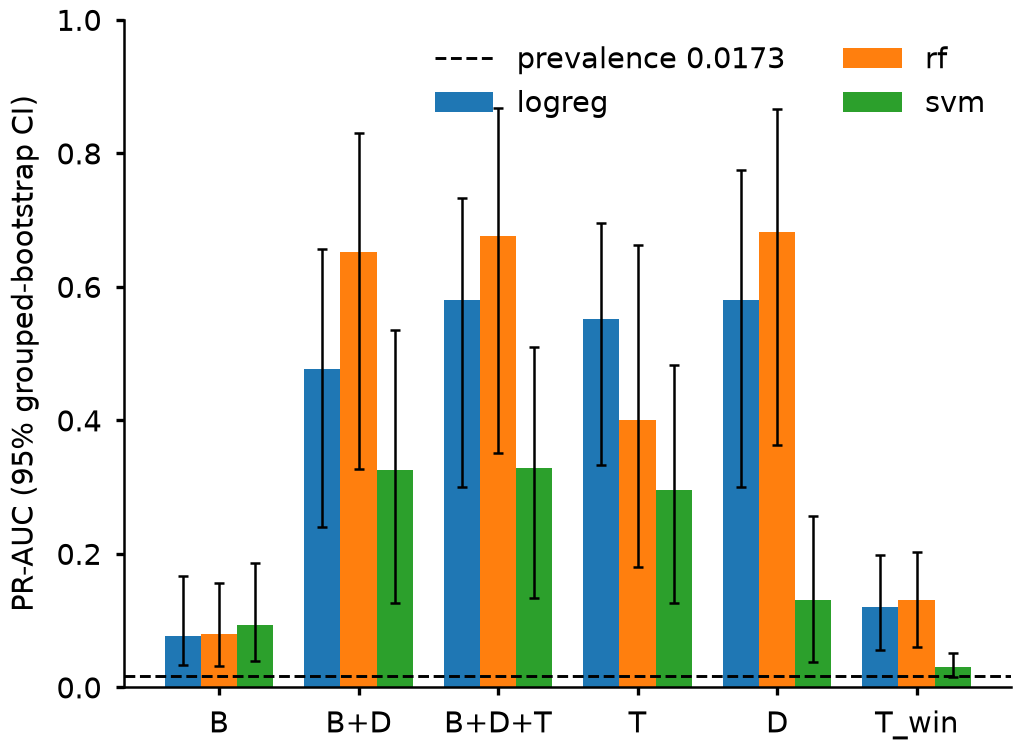
\includegraphics[width=\columnwidth]{figures/f3_hi_pr_auc.png}
\caption{IBM HI-Small (itself synthetic), primary variant (ambiguous candidates excluded): PR-AUC of the pre-specified feature sets B, B+D, B+D+T and T, and of the controls D and $T_{\mathrm{win}}$ (exploratory), for logistic regression (logreg), random forest (rf) and RBF-SVM (svm). Prevalence 0.0173 (dashed line), 131 positives in 14 positive groups. Error bars: 95\% percentile CI of a grouped bootstrap over groups. Pooled out-of-fold, mean of 5 repeats. Three exploratory ablations (B+D+T\_local, B+D+T\_win, T\_local) are omitted; see text.}
\label{fig:hi}
\end{figure}

\subsection{No detectable topological lift on IBM data}
The pre-specified primary comparison is in Table~\ref{tab:paired}. On HI-Small (14 positive groups) B+D+T minus B+D is +0.104 [\mi0.002, +0.171] for LR, +0.025 [\mi0.050, +0.102] for RF and +0.003 [\mi0.111, +0.077] for SVM; every interval includes 0. On LI-Small (10 positive groups) it is +0.033 [\mi0.007, +0.097] (LR), \mi0.012 [\mi0.119, +0.077] (RF) and \mi0.044 [\mi0.181, +0.091] (SVM); again every interval includes 0. The two datasets agree in that every interval includes 0; the point estimates differ in sign for RF and SVM (positive on HI-Small, negative on LI-Small) and are small, but with 14 and 10 positive groups a small positive effect and a small negative one are both compatible with the data. This is a statement of low power, not of absence.

The conclusion does not depend on how ambiguous candidates are counted. With ambiguous candidates counted positive, HI-Small has prevalence 0.0805 and 142 positive groups, and B+D+T minus B+D is +0.027 [\mi0.015, +0.086] (LR), +0.003 [\mi0.056, +0.032] (RF) and +0.176 [\mi0.033, +0.297] (SVM); LI-Small has prevalence 0.0513 and 189 positive groups, and the differences are \mi0.001 [\mi0.014, +0.008], +0.003 [\mi0.003, +0.008] and +0.007 [\mi0.009, +0.028]. All six intervals include 0.

\begin{table*}[t]
\caption{Paired PR-AUC differences [95\% grouped-bootstrap CI over groups, same resamples for both feature sets]. Primary (pre-specified): B+D+T minus B+D. Secondary (pre-specified): B+D minus B. IBM AMLworld is itself synthetic. HI-Small: 14 positive groups; LI-Small: 10; synthetic conditions: 46, 46, 55 and 52 positive groups (Table~\ref{tab:data}); transfer: one model per direction, CI over test groups (HI$\to$LI: 10; LI$\to$HI: 14).}
\label{tab:paired}
\centering
\footnotesize
\setlength{\tabcolsep}{4pt}
\begin{tabular}{@{}llccc@{}}
\toprule
Dataset & Comparison & LR & RF & SVM \\
\midrule
HI-Small & primary & +0.104 [\mi0.002, +0.171] & +0.025 [\mi0.050, +0.102] & +0.003 [\mi0.111, +0.077] \\
LI-Small & primary & +0.033 [\mi0.007, +0.097] & \mi0.012 [\mi0.119, +0.077] & \mi0.044 [\mi0.181, +0.091] \\
Transfer HI$\to$LI & primary & \mi0.017 [\mi0.147, +0.092] & \mi0.066 [\mi0.177, \mi0.012] & \mi0.050 [\mi0.142, +0.042] \\
Transfer LI$\to$HI & primary & \mi0.276 [\mi0.550, \mi0.036] & \mi0.019 [\mi0.079, +0.046] & \mi0.056 [\mi0.123, +0.025] \\
Synth.\ hn off, chords default & primary & +0.018 [+0.002, +0.057] & +0.038 [+0.010, +0.095] & +0.077 [+0.019, +0.175] \\
Synth.\ hn off, chords off & primary & +0.030 [+0.010, +0.074] & +0.043 [+0.011, +0.110] & +0.096 [+0.029, +0.210] \\
Synth.\ hn on, chords default & primary & +0.005 [\mi0.009, +0.021] & \mi0.003 [\mi0.012, +0.004] & +0.038 [\mi0.004, +0.080] \\
Synth.\ hn on, chords off & primary & +0.014 [\mi0.006, +0.039] & +0.003 [\mi0.004, +0.012] & +0.052 [+0.001, +0.109] \\
\midrule
HI-Small & secondary & +0.399 [+0.139, +0.571] & +0.572 [+0.276, +0.720] & +0.233 [+0.057, +0.379] \\
LI-Small & secondary & +0.072 [+0.020, +0.173] & +0.132 [+0.045, +0.283] & +0.105 [\mi0.060, +0.276] \\
Synth.\ hn off, chords default & secondary & +0.440 [+0.324, +0.535] & +0.383 [+0.265, +0.477] & +0.411 [+0.213, +0.520] \\
Synth.\ hn off, chords off & secondary & +0.414 [+0.290, +0.509] & +0.389 [+0.248, +0.519] & +0.368 [+0.184, +0.487] \\
Synth.\ hn on, chords default & secondary & +0.542 [+0.418, +0.621] & +0.389 [+0.258, +0.494] & +0.598 [+0.458, +0.676] \\
Synth.\ hn on, chords off & secondary & +0.510 [+0.376, +0.600] & +0.395 [+0.244, +0.513] & +0.614 [+0.468, +0.698] \\
\bottomrule
\end{tabular}
\end{table*}

\subsection{Synthetic data: a small lift that does not carry over}
On the synthetic generator B+D is already high (0.960 to 0.983 for LR, 0.956 to 0.997 for RF and 0.874 to 0.937 for SVM over the four conditions), and the generator is nearly separable by D alone. B+D+T minus B+D has an interval above 0 in 7 of the 12 condition-model cells (Table~\ref{tab:paired}): all three models with hard negatives off, and only the SVM, with chords off, with hard negatives on (+0.052 [+0.001, +0.109]). For hard negatives off and default chords, B+D scores 0.970 (LR), 0.959 (RF) and 0.892 (SVM) and B+D+T 0.988, 0.996 and 0.969. The gain is small, and it does not appear on IBM: for the pre-specified comparison no IBM cell (HI-Small, LI-Small or transfer) has an interval above 0. Two exploratory ablation cells on HI-Small do (B+D+$T_{\mathrm{local}}$ with LR, +0.141 [+0.031, +0.224]; B+D+$T_{\mathrm{win}}$ with SVM, +0.088 [+0.006, +0.176]); they are uncorrected for multiplicity, and the same ablations have intervals that include 0 on LI-Small.

The gain is also not concentrated where the design predicted (exploratory, per scenario; Fig.~\ref{fig:lift}). Topology was expected to be nearly redundant for isolated rings and to matter for rings whose loops are filled, split or crowded by their neighbourhood. Yet, counting model-condition cells whose interval lies above 0 (intervals are plotted in Fig.~\ref{fig:lift}), isolated rings show 8 of 12 (SVM in all four), dense rings in 2 of 12 (only with internal chords off and hard negatives off: LR +0.130 [+0.038, +0.330], RF +0.123 [+0.029, +0.329]), and chorded rings in 6 of 12 (SVM 4 of 4, RF 2 of 4, LR 0 of 4). The per-scenario groups are few (39 isolated, 10 dense, 8 chorded at hard negatives off with default chords), and the cause is untested: $T$ also encodes neighbourhood size and degree structure, and the generator may have artefacts. When the planted shortcut-filled pseudo-rings are ranked, adding $T$ lowers their mean out-of-fold percentile under logistic regression (B+D 0.982, B+D+T 0.909, with hard negatives off; descriptive means with no interval), consistent with, but not proof of, the intended effect.

\begin{figure*}[t]
\centering
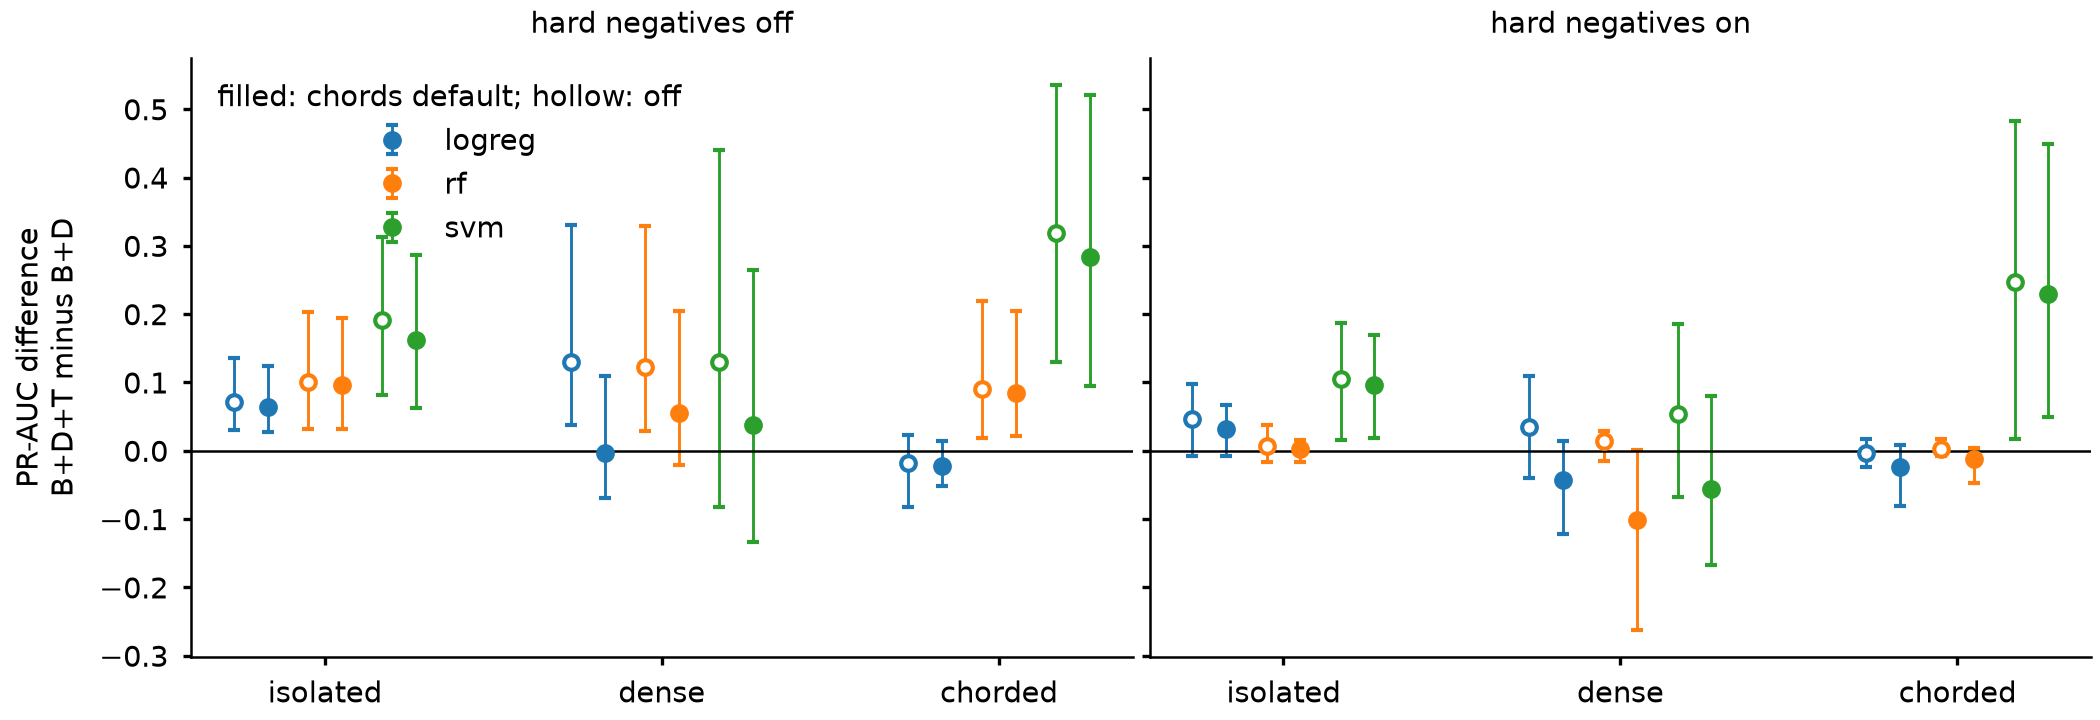
\includegraphics[width=\textwidth]{figures/f4_lift_per_scenario.png}
\caption{Exploratory. Synthetic data, six seeds pooled: paired PR-AUC difference B+D+T minus B+D per scenario for logistic regression, random forest and RBF-SVM, hard negatives off (left) and on (right); filled markers: dense\_internal\_chords default, hollow: off. Error bars: 95\% percentile CI of a grouped bootstrap over groups (same resamples for both feature sets). Each scenario's positives are compared with all negatives, so prevalence differs per scenario: isolated 0.0108 to 0.0265, dense 0.0048 to 0.0113, chorded 0.0050 to 0.0118; positive groups per scenario at hard negatives off with default chords: isolated 39, dense 10, chorded 8.}
\label{fig:lift}
\end{figure*}

\subsection{Transfer and the ring-birth signal}
Training on one IBM dataset and testing on the other (labelled transfer; one model per direction) gives B+D PR-AUC of 0.133, 0.149 and 0.124 for LR, RF and SVM from HI to LI at prevalence 0.0039. B+D+T minus B+D is again not above 0 in any cell (Table~\ref{tab:paired}); it is below 0 for RF from HI to LI (\mi0.066 [\mi0.177, \mi0.012]) and for LR from LI to HI (\mi0.276 [\mi0.550, \mi0.036]). Ring birth by itself, ranked without any model (\texttt{\mi D\_birth}), scores 0.314 [0.097, 0.487] on HI-Small at prevalence 0.0173 but 0.006 [0.002, 0.025] on LI-Small, which is not distinguishable from that dataset's prevalence of 0.0039. The signal seen on HI-Small therefore does not replicate on LI-Small. The two values are separate within-dataset scores of a model-free ranking, not a transfer result.

\subsection{Exploratory ablations}
The topological set splits into local and window parts. With HI-Small, B+D+$T_{\mathrm{local}}$ minus B+D is +0.141 [+0.031, +0.224] for LR, +0.041 [\mi0.037, +0.106] for RF and +0.037 [\mi0.081, +0.126] for SVM, while B+D+$T_{\mathrm{win}}$ minus B+D is +0.034 [\mi0.005, +0.094], +0.007 [\mi0.025, +0.059] and +0.088 [+0.006, +0.176]. These were added after the first run, are one model each and are not corrected for multiplicity. As a control, $T_{\mathrm{win}}$ alone scores 0.121 [0.056, 0.198] (LR) and 0.130 [0.061, 0.202] (RF) on HI-Small at prevalence 0.0173 although it is constant within a window; a time proxy is consistent with this but was not tested, and on LI-Small the same sets score 0.006 and 0.004 at prevalence 0.0039. Among the infinite-bar caps fixed in advance (window maximum, fixed 1.0, 1.1 times the window maximum) the largest absolute paired difference to the default is 0.024 (SVM, B+D+T, HI-Small; fixed 1.0 against the window maximum, \mi0.024 [\mi0.037, \mi0.004]). A cap based on the local maximum, examined after seeing results, changes the HI-Small SVM B+D+T value by +0.190 [+0.097, +0.240]; it is post hoc, from one model, and not adopted (Appendix~\ref{app:expl}).

\subsection{Candidate recall}
Candidate generation caps what any classifier can find (Table~\ref{tab:recall}). In the first HI-Small window (days 0--5), 15 CYCLE attempts are complete, 11 involve at most 6 accounts, and 8 of those are recovered at $\tau$ quantile 0.05 (6 also carry a positive CYCLE label under the 80\% rule). On the whole HI-Small data, 19 of 34 reachable attempts are recovered. On the synthetic generator with hard negatives off, recall of planted rings is 1.00 at every $\tau$ tested; with hard negatives on it is lower at $\tau=0.05$ (0.52 isolated, 0.21 dense, 0.42 chorded), 1.00 at 0.15 to 0.25, and limited by the enumeration cap above.

\begin{table}[t]
\caption{Candidate recall of complete CYCLE attempts on IBM data, $\tau$ quantile 0.05, maximum ring length 6. ``Reachable'' means at most 6 accounts. ``Recovered'' means a candidate with exactly the attempt's account set; ``labelled'' adds that the candidate carries a positive CYCLE label. Counts, not a sample: no interval. LI days 0--5 contains one complete attempt.}
\label{tab:recall}
\centering
\small
\begin{tabular}{@{}llrrrr@{}}
\toprule
Data & Scope & Complete & Reachable & Recovered & Labelled \\
\midrule
HI & days 0--5 & 15 & 11 & 8 & 6 \\
HI & whole data & 54 & 34 & 19 & 15 \\
LI & whole data & 12 & 6 & 3 & 3 \\
\bottomrule
\end{tabular}
\end{table}

\subsection{Audit of the weights on IBM patterns}
For HI-Small windows 0 and 2 pooled, the edge-level AUC of CYCLE pairs against background pairs is 0.794 for the combined weight, which is built from rank-normalised scores. For the raw scores it is 0.795 for balance and 0.601 for timing; for the rank-normalised scores it is 0.804 and 0.589. The RANDOM pattern type has a similar weight AUC (0.785), and the other attempt types range from 0.528 to 0.653. About 0.899 of CYCLE pairs have fewer than three payments, so their timing score is the imputed median, against 0.467 of background pairs. The wash-trading weights therefore describe IBM cycles only partly, mostly through balance, which is why IBM is used to test the machinery.

\subsection{Adaptive thresholds}
On the drift stream of the optimization report (40 windows, six stream seeds, $\lambda=1$, lag $d=2$), the share of the hindsight-oracle reward is 0.298 $\pm$ 0.059 for a fixed threshold, 0.861 $\pm$ 0.020 for re-tuning every 5 windows, and 0.981 $\pm$ 0.006 for online gradient ascent (Table~\ref{tab:bandit}). The bandits lose: discounted UCB is \mi1.245 $\pm$ 1.066 below the re-tuned comparator (0 of 6 seeds better) and sliding-window Thompson sampling \mi0.771 $\pm$ 0.744 below (2 of 6). The only positive cell is discounted UCB at lag 5 ($+0.258$, all 6 seeds), which is not a skill result: on stream seed 0 that policy never played the last arm within its 35 windows. In this stream a single play of the arm that flags almost everything costs about as much as the whole oracle total, and rewards are clipped at $\pm10$ before the policies see them, which hides its size. Pre-set hyperparameters were not tuned after seeing results; a later sensitivity run with a larger discount did better and was not adopted. This is one simulated synthetic stream and does not show that bandits are poor in general.

\begin{table}[t]
\caption{Threshold policies on the synthetic drift stream of the optimization report: share of hindsight-oracle cumulative reward at $\lambda=1$, lag $d=2$ (mean $\pm$ std over 6 stream seeds; not a CI), and paired difference of the bandits against re-tuning every 5 windows (retune$_5$), with the number of seeds on which the bandit is better. Synthetic only.}
\label{tab:bandit}
\centering
\small
\begin{tabular}{@{}lcc@{}}
\toprule
Policy & Share of oracle & Minus retune$_5$ \\
\midrule
Fixed & 0.298 $\pm$ 0.059 & \\
Re-tune every 5 windows & 0.861 $\pm$ 0.020 & \\
Online gradient ascent & 0.981 $\pm$ 0.006 & \\
Discounted UCB & \mi0.383 $\pm$ 1.067 & \mi1.245 $\pm$ 1.066 (0/6) \\
Sliding-window Thompson & 0.091 $\pm$ 0.753 & \mi0.771 $\pm$ 0.744 (2/6) \\
\bottomrule
\end{tabular}
\end{table}

\subsection{Other exploratory studies}
Three further studies are exploratory and summarized in Appendix~\ref{app:expl}. A next-window severity regression on synthetic rings (IBM has no next-window wash volume) recovers generator structure: ring length alone has a root-mean-square error of 0.132 [0.125, 0.139] for random forest against 0.141 [0.134, 0.149] for B+D, and $T$ adds nothing. Ward clustering of positive IBM rings agrees only weakly with pattern types (HI-Small, $k=4$: adjusted Rand index 0.097 against 0.398 against group identity), so the clusters track attempts more than types; the bootstrap intervals for this study are biased and are not used. A synthetic pump-and-dump track with no topology shows that the harness runs on a second pattern type, and the generator is nearly separable by exit timing.

%--------------------------------------------------------------------
\section{Discussion and Limitations}
\label{sec:discussion}

\textbf{What the evidence supports.} Direction and behaviour features, which include the ring birth that the filtration produces, carry the detection signal on every dataset we tried. The topological increment, measured by a comparison fixed in advance, is not detectable within either IBM dataset (itself synthetic), where the intervals are compatible with small effects of either sign; in transfer between the datasets two primary cells are negative with intervals that exclude 0. The synthetic generator, built so that topology should matter, shows a small gain in 7 of 12 cells, but the gain is not where the design predicted, the generator is nearly separable by D, and IBM shows nothing comparable. We therefore do not claim that topology improves detection on real wash-trading data, and the results do not say that it fails to; they say that this experiment cannot tell.

\textbf{Reading the null result.} The width of the IBM intervals is set by the number of positive groups, not by the number of positive rings, which is why 131 positive candidates give only 14 groups. Every within-dataset interval for the primary comparison (HI-Small and LI-Small) therefore contains 0, and the largest upper bound is +0.171 (logistic regression, HI-Small), so effects of either sign of that order remain compatible with the data there. In the HI--LI transfer, two primary cells are negative with intervals that exclude 0 (HI to LI, RF \mi0.066 [\mi0.177, \mi0.012]; LI to HI, LR \mi0.276 [\mi0.550, \mi0.036]). We can offer hypotheses for why topology adds little, and label them as untested: ring birth, which the filtration produces, already sits in D; the baseline sees the full window graph; and for isolated rings persistence repeats enumeration. The exploratory local-topology gain for logistic regression on HI-Small does not replicate on LI-Small (B+D+$T_{\mathrm{local}}$ minus B+D $+0.002$ [\mi0.033, +0.042]), and the window-level set is where a time proxy would act. None of this changes the primary result.

\textbf{Cost.} Whether persistence features justify their computational cost is not settled by this study; we did not measure a cost-benefit trade-off.

\textbf{Limitations.}
\begin{enumerate}
\item \emph{Few positive groups.} The effective sample size is the number of positive groups: 14 on HI-Small (131 positive candidates) and 10 on LI-Small (38). In 144 of 150 fold-repeats over three $\tau$ values, the two datasets, five folds and five repeats, a fold holds fewer than 5 positive groups. Intervals are wide and nothing was tuned to narrow them. LI-Small has only 3 CYCLE positives, so a cycle-only analysis is unusable there.
\item \emph{HI and LI disagree.} The ring-birth detector works on HI-Small and not on LI-Small, which shows how fragile a single-dataset signal is.
\item \emph{Time proxy.} Window-constant features alone score above chance on HI-Small; we did not test the explanation.
\item \emph{Synthetic data.} Both IBM datasets and our own generator are synthetic. The generator's designer decides what separates hard negatives from rings; with hard negatives on, 0.963 (chords default) and 0.972 (chords off) of all candidates are ambiguous.
\item \emph{Weights and imputation.} The scores encode wash-trading behaviour, and 0.685 to 0.966 of each laundering group's pairs have an imputed timing score. IBM amounts mix currencies. IBM data are not market transactions.
\item \emph{Candidate recall.} Only 11 of 15 complete HI cycle attempts in the first window can be reached with at most 6 accounts, and the bounded-enumeration algorithm has a published caveat \cite{bauernoppel2025bounded}.
\item \emph{Sampled betweenness.} On IBM windows betweenness uses 100 sampled sources, so most nodes score 0 (0.1594 of the 404{,}273 nodes of the first HI window are non-zero).
\item \emph{Untuned SVM and no GNN.} The SVM has fixed hyperparameters and is weaker than the random forest on HI-Small (B+D 0.326 against 0.652). No graph neural network, community-detection or published topological method was run, so we make no claim of outperforming any of them.
\item \emph{Multiplicity.} 495 paired rows were computed with no correction; the exploratory ablations in particular should be read as hypotheses.
\item \emph{Threshold study.} It uses one simulated drift stream and a fixed arm grid and reward clipping; bandit hyperparameters were set in advance.
\end{enumerate}

\textbf{What was not done.} The planned NFT experiment on real wash-trade labels was not run: running queries on Dune is blocked on its free tier. BigQuery access was confirmed and the schemas inspected; the planned leakage-controlled subset would use only the proxy-label filters that are not cycle rules, because two of the five filters of the public Dune wash-trade model (as inspected by us) are cycle-type rules and would leak the structure our method detects. We also did not run an undirected clique-complex ablation, so the benefit of the directed construction is argued from construction (and checked on toy graphs), not measured; a persistence-image ablation; classifiers on single-score filtrations; or sweeps over window length, stride, label threshold and, for classification, $\tau$ and maximum ring length (only candidate recall was swept). A real-data pump-and-dump experiment is likewise absent. Finally, the time-ordered evaluation planned in the design was unusable (Section~\ref{sec:setup}), so the out-of-sample evidence is transfer between two datasets from the same generator.

\textbf{Deviations from the design.} De-duplication keeps the shortest ring first and then the lowest birth, and removes nothing for lengths up to 9; the optimization report keeps a maximum length of 5 and a fixed cap of 1.0 for its legacy topological columns while the classification uses 6 and the window-maximum cap; timing is imputed for pairs with fewer than three payments, not only for a single payment; a cycle-only subset and the ambiguous-counted-positive variant were added; and the planned false-positive rate at 80\% recall was replaced by the rank percentile of each negative kind.

\textbf{Ethics.} A ring score is a suspicion score, not a finding of guilt. Publishing the scores may help adversaries who inject decoy trades to break balance or regularity.

%--------------------------------------------------------------------
\section{Conclusion and Future Work}
\label{sec:conclusion}

We built and tested a pipeline that localizes candidate rings exactly and describes each by direction and behaviour features, graph baseline features and persistent homology of a directed flag complex, and we compared B+D+T with B+D under a protocol fixed in advance. Direction and behaviour features carry the signal. On IBM AML data (itself synthetic) topology adds no detectable lift within either dataset, with intervals that cannot exclude a small effect of either sign given 14 and 10 positive groups, and two of six transfer cells are negative with intervals that exclude 0; on a nearly separable synthetic generator it adds a small lift that does not carry over; the ring-birth signal seen on HI-Small does not replicate on LI-Small; and bandit thresholds lose to periodic re-tuning in our simulation. Future work includes the NFT experiment on the cycle-free subset of proxy labels, an undirected clique-complex ablation, persistence-image and learned-vectorization ablations, sweeps over the parameters listed above, more positive groups through larger IBM variants, and a test of whether the window-level features act as a time proxy.

%--------------------------------------------------------------------
\bibliographystyle{IEEEtran}
\bibliography{refs}

%--------------------------------------------------------------------
\appendices

\section{Optimization-report results (pinned generator)}
\label{app:report}
These numbers come from the optimization report on its pinned synthetic generator (dense, chorded, shortcut-filled and hot-wallet counts set to 0; ambiguous candidates counted as negatives), not from IBM data. Ring-birth detector test average precision rises from 0.5675 with equal weights to 0.9997 with weights learned on the simplex, (0.0, 0.2067, 0.7933) for (reciprocity, balance, regularity); learning matters because of Proposition~1. A logistic classifier on D reaches test average precision 0.9984 and with the legacy topological columns 0.9969, so topology does not help the report's detector either. Gradient descent with a step matched to the local curvature reaches an optimality gap of $10^{-6}$ in 322 iterations. On the 40-window drift stream, cumulative reward after warm-up as a share of the oracle is 0.2367 for a fixed threshold, 0.86 for re-tuning every 5 windows and 0.97 for online gradient ascent. Seed 0 of the bandit benchmark reproduces the report's stream exactly (fixed 71.0, re-tune 258.0, ascent 291.0, oracle 300.0).

\section{Exploratory results}
\label{app:expl}
\begin{table}[h]
\caption{Exploratory side studies. Severity and pump-and-dump are synthetic only. Clustering uses IBM HI-Small positive rings (131 rings in 14 groups; $k=4$, $D$ plus $T_{\mathrm{local}}$ landscape). Percentile CIs of the clustering bootstrap are biased and not used. No multiplicity correction.}
\label{tab:expl}
\centering
\footnotesize
\setlength{\tabcolsep}{3pt}
\begin{tabular}{@{}p{0.34\columnwidth}p{0.58\columnwidth}@{}}
\toprule
Study & Result \\
\midrule
Severity, RMSE (random forest) & B+D 0.141 [0.134, 0.149]; $D_{\mathrm{length}}$ alone 0.132 [0.125, 0.139]; fair persistence fit 0.221 [0.203, 0.237]; B+D+T minus B+D $\mi$0.001 [$\mi$0.004, +0.002]; random-forest importance of \texttt{D\_length} 0.796 \\
Clustering, HI & ARI against type 0.097 (random 0.000); against group id 0.398; purity 0.489 (random 0.365, majority 0.336) \\
Clustering, LI ($T_{\mathrm{local}}$ landscape, $k=3$, 9 groups) & ARI 0.260; purity 0.730 (random 0.536, majority 0.459) \\
Pump-and-dump, default exits (47 positive groups, prevalence 0.390) & M features 0.890 (LR), 0.976 (RF), 0.928 (SVM) against group-size baseline 0.388, 0.375, 0.414; \texttt{\mi M\_exit\_spread\_h} alone 0.906 [0.860, 0.945]; with wider exits 0.643 [0.513, 0.752] \\
Cap, HI SVM B+D+T & window maximum 0.329; fixed 1.0 0.305; $1.1\times$ maximum 0.334; local maximum (post hoc) 0.518 \\
\bottomrule
\end{tabular}
\end{table}

\section{Reproduction}
Every number in this paper was read from stored result files by a script that records its source; the stored seeds are cross-validation seed 0, bootstrap seed 12345, model seed 0 and synthetic seeds 0 to 5. The pre-existing optimization-report outputs are never overwritten. The test suite collects 210 tests; model performance is never a test.

\end{document}
